\documentclass[a4paper]{article}
\usepackage{iwslt15,amssymb,amsmath,epsfig}
\usepackage{csquotes}
\usepackage{algorithm}
\usepackage[hyphens]{url}
\usepackage{hyperref}
\hypersetup{breaklinks=true}
\usepackage{listings}
\usepackage{graphicx}
\usepackage{subcaption}
\lstset{
     breaklines=true,
     basicstyle=\ttfamily
}

\bibliographystyle{IEEEtran}
\setcounter{page}{1}
\sloppy		% better line breaks
%\ninept

\newcommand{\ts}{\textsuperscript}

\title{Hand Gesture Recognition with Convolutional Neural Networks}

%%%%%%%%%%%%%%%%%%%%%%%%%%%%%%%%%%%%%%%%%%%%%%%%%%%%%%%%%%%%%%%%%%%%%%%%%%
%% If multiple authors, uncomment and edit the lines shown below.       %%
%% Note that each line must be emphasized {\em } by itself.             %%
%% (by Stephen Martucci, author of spconf.sty).                         %%
%%%%%%%%%%%%%%%%%%%%%%%%%%%%%%%%%%%%%%%%%%%%%%%%%%%%%%%%%%%%%%%%%%%%%%%%%%
\makeatletter
\def\name#1{\gdef\@name{#1\\}}
\makeatother
\name{{\em Benjamin Alt, Lukas Hennig, Felix Hertlein}}
%%%%%%%%%%%%%%% End of required multiple authors changes %%%%%%%%%%%%%%%%%

\address{Interactive Systems Lab, Institute for Anthropomatics and Robotics\\
Karlsruhe Institute of Technology, Germany\\
{\small \tt benjamin.alt@student.kit.edu}\\
{\small \tt lukas.hennig@student.kit.edu}\\
{\small \tt felix.hertlein@student.kit.edu}
}
%
\begin{document}
\maketitle
%
\begin{abstract}
Robust systems for automatic hand gesture recognition have numerous applications in disability assistance, gesture-based user interfaces and gaming. We propose an approach for classifying hand gestures from American Sign Language (ASL) based on convolutional neural networks. To that end, we designed and implemented a deep convolutional neural network architecture and trained it on the \enquote{Sign Language MNIST} dataset. Additionally, we evaluated the generalization capacity of our network on a custom dataset and analyzed it by visualizing the learned features.
\end{abstract}

\section{Introduction}

Applications:
- Disability assistance
- Natural User Interfaces (NUIs)
- Games

Tools:
- Pytorch: Built-in modules for dataset loading, layers, activations, optimizers, .., automatic differentiation (easy)
- Kaggle, Google Colab, Lab clusters: Grdis search for optimal hyperparameters

Training only took a few minutes: Allowed for fast prototyping and training at home

\section{Dataset}

- Sign language MNIST
- Can be found online
- Images of hand poses corresponding to the American Sign language alphabet, except letters J and Z because they require motion for their representation
- Grayscale, 28x28 pixels, similar to classical Digit Recognition MNIST dataset
- One class per letter: 26 classes, but only images for 24 of those, labels 0-25
- Training set: 27455 images, Test set: 7172 images
- Dataset relies heavily on data augmentation:
  - Original images: 1794 RGB, by 7 different users
  - Not much variation in those original images: similar hand poses, lightning conditions, backgrounds, ..
  - Preparation: Cropping to hand, resizing, grayscaling
  - Data augmentation by dataset creators: 50+ variations
    - Different filters, Random noise, brightness and contrast variations, small amounts of random rotation
  - Own data augmentation:
    - Random rotation, random horizontal flip (left-handed), Random crop (random position, aspect ratio and slightly smaller size, resized to 28 by 28)

We trained our neural networks with images from the \textit{Sign Language MNIST} dataset \cite{DatasetKaggle}. Similar to the classical Digit Recognition MNIST dataset \cite{MNIST}, the images are 28 by 28 pixels in size with one grayscale value between 0 and 255 per pixel. Each image depicts a hand gesture corresponding to one letter in the American Sign Language alphabet. Therefore there are 26 different classes with labels from 0 to 25. But since the letters J and Z require motion to be represented, the dataset doesn't contain images for those two letters. Consequently our neural network only recognizes 24 of those 26 classes.

The original color images were cropped to only contain the hand and then grayscaled and downscaled to 28 by 28 pixels. The cropped original color images for the different letters can be seen in figure \ref{fig:full_colored}. The corresponding downscaled grayscale images are shown in figure \ref{fig:full_grayscale}.

The dataset is split into a training set with 27455 images and a separate test set with 7172 images. We use the images from the training set to train our neural networks and then determine recognition rates with the images from the test set.

The creators of the dataset heavily relied on data augmentation: They started with 1794 original RGB images that were taken by only 7 different users repeating the various hand gestures. There is not much variation in those original images regarding the hand poses, lightning conditions and backgrounds. Those images were cropped to only contain the hand and then grayscaled and downscaled to 28 by 28 pixels.

and then applied over 50 variations of different image transformations. Those transformations include 






\begin{figure}
     \centering
     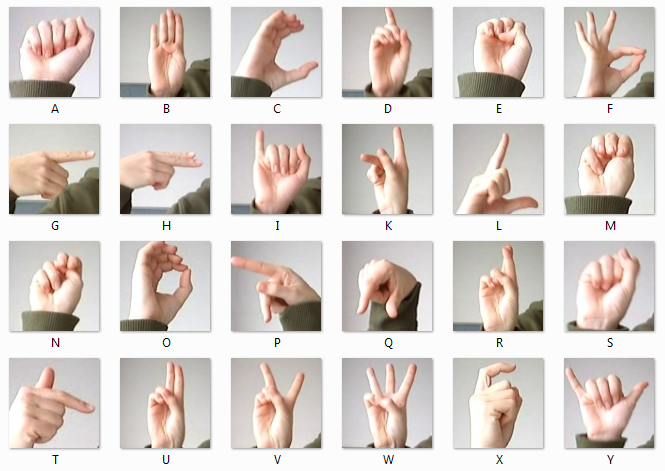
\includegraphics[width=1\linewidth]{graphics/dataset/amer_sign2.png}
     \caption{\textit{Cropped original color images of hand gestures corresponding to the American Sign Language alphabet \cite{DatasetKaggle}}}
     \label{fig:full_colored}
\end{figure}

\begin{figure}
     \centering
     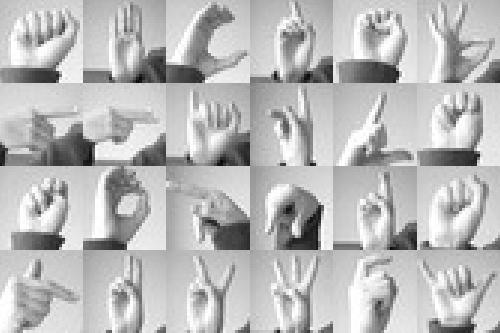
\includegraphics[width=1\linewidth]{graphics/dataset/amer_sign3.png}
     \caption{\textit{Downscaled grayscale images from the dataset \cite{DatasetKaggle}}}
     \label{fig:full_grayscale}
\end{figure}

%\begin{figure}
%     \centering
%     \begin{tabular}{cc}
%          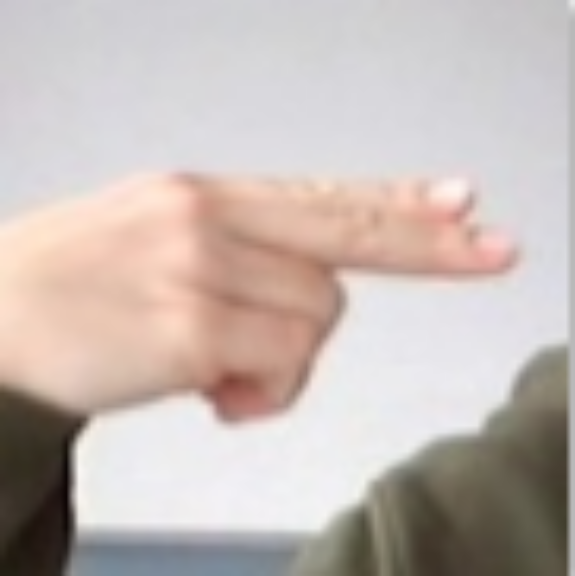
\includegraphics[width=.35\linewidth]{graphics/dataset/colored.png}&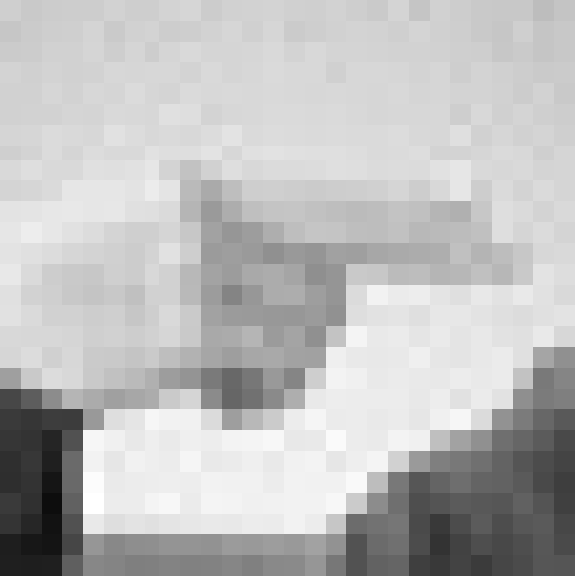
\includegraphics[width=.35\linewidth]{graphics/dataset/grayscale.png}
%     \end{tabular}
%     \caption{\textit{Original cropped colored image (left) and corresponding grayscale image with noise (right)}}
%     \label{fig:colored}
%\end{figure}

\begin{figure}
     \centering
     \begin{tabular}{cc}
          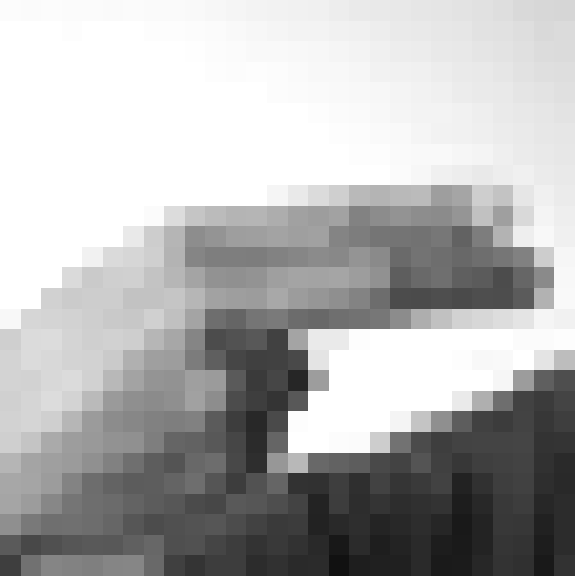
\includegraphics[width=.35\linewidth]{graphics/dataset/bright.png}&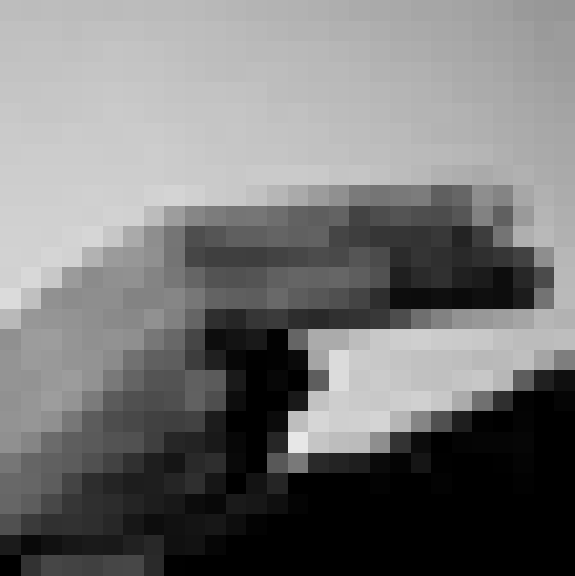
\includegraphics[width=.35\linewidth]{graphics/dataset/dark.png}
     \end{tabular}
     \caption{\textit{Variations of brightness}}
     \label{fig:brightness}
\end{figure}

\section{Models}

In order to solve this task, we designed various deep learning models and evaluated them using the test dataset. Each model consists of a convolutional neural network (CNN) followed by a fully connected neural network. During the process of development, we increased the complexity of our nets beginning with the SimpleCNN (see section \ref{sec:simpleCNN}). As the successor we propose a net called  DeepCNN in section \ref{sec:deepCNN}. We improved the results of the DeepCNN by augmenting the training data and adding regularization technique (section \ref{sec:deepCNN_augmented} and \ref{sec:deepCNN_regularized}).

\subsection{SimpleCNN}\label{sec:simpleCNN}

\begin{figure*}
    \centering
    \begin{subfigure}[b]{0.2\textwidth}
        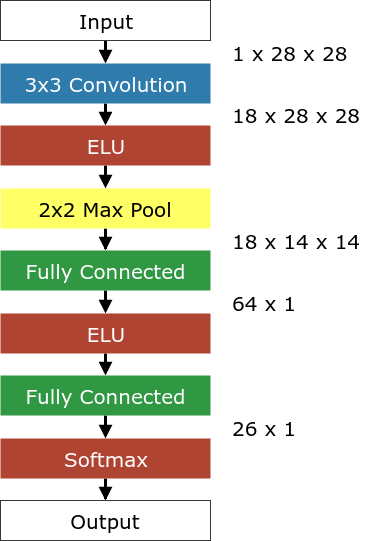
\includegraphics[height=0.25\paperwidth]{graphics/nets/SimpleCNN}
        \caption{\textit{Model of SimpleCNN}}
        \label{fig:simpleCNN_model}
    \end{subfigure}
    \qquad
    \qquad
    \begin{subfigure}[b]{0.6\textwidth}
        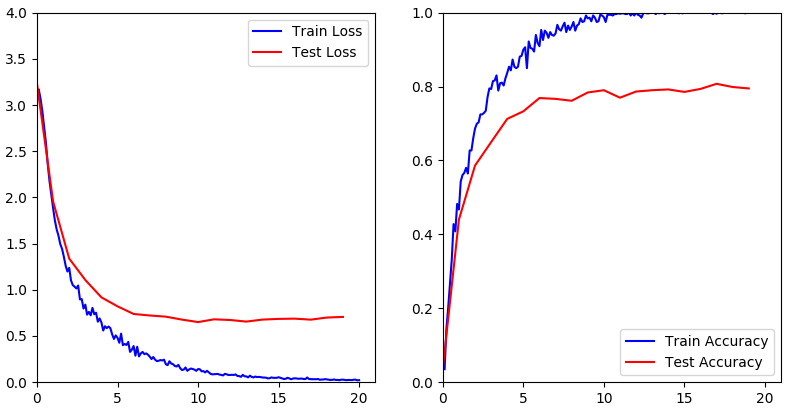
\includegraphics[height=0.25\paperwidth]{graphics/nets/SimpleCNN_Results}
        \caption{\textit{Results on SimpleCNN}}
        \label{fig:simpleCNN_results}
    \end{subfigure}
    \caption{\textit{Subplot \ref{fig:simpleCNN_model} visualizes all layers of the SimpleCNN model. Subplot \ref{fig:simpleCNN_results} displays the train and test losses (left plot), as well as the train and test accuracies (right plot) as a function of the trained epochs.}}\label{fig:simpleCNN}
\end{figure*}

In our first attempt we designed a basic model to classify the hand gestures, called the SimpleCNN. Figure \ref{fig:simpleCNN_model} visualizes the overall structure. This model takes a tensor of the dimensions 1x28x28 as an input since the data consists of 28x28 pixels grayscale images. The images are processed by a convolution layer with the kernel size of 3x3 and zero padding, thus it does not reduce the last two dimensions. Afterwards an exponential linear unit (ELU, \cite{clevert2015fast}) is applied as an activation function with $\alpha = 1$.
\vspace{-0.2cm}

\begin{equation}\label{eq:elu}
f(x) = \left\{\begin{alignedat}{2}
    & x && \qquad \text{if} \quad x < 0\\
    & \alpha \cdot (e^x - 1) && \qquad \text{if} \quad x >= 0\\
  \end{alignedat}\right.
\end{equation}

The ELU has some advantages over the widely used activation function Rectified Linear Unit (ReLU). By design, the ELU function (equation \ref{eq:elu}) is smooth and can produce negative values. For this reason, the mean of all activations is closer to zero, which results in a faster learning \cite{clever2015fast}.
The resulting activation is processed by a 2x2 max pooling layer in order to reduce the dimensionality. Subsequently, we applied two fully connected layer with an ELU function in-between and a Softmax activation function at the end. This results in a probability distribution of 26 classes, one class per character. Due to the fact, that the letters J and Z need motion to be recognized, they are not part of the training set. The activation for those two classes is presumably close to zero after training for all inputs.

We used the Adam optimizer \cite{Kingma2014} in conjunction with mini batch training with a batch size of 512 instances. The optimizer minimized the cross-entropy error with L2 regularization between our output vector and the ground truth vector. 
Figure \ref{fig:simpleCNN_results} shows the development of the training and test losses, as well as the training and test accuracies throughout the training process. The test loss curve (red) indicates, that after 10 epochs the net stops to learn generalized features. The training loss decreases further until it reaches zero. This suggests, that the net is memorizing the training data without losing its generalization. We achieved a train accuracy of 80.7 \% after 20 epochs.

\subsection{DeepCNN}\label{sec:deepCNN}

\begin{figure*}
    \centering
    \hspace{-1cm}
    \begin{subfigure}[b]{0.4\textwidth}
        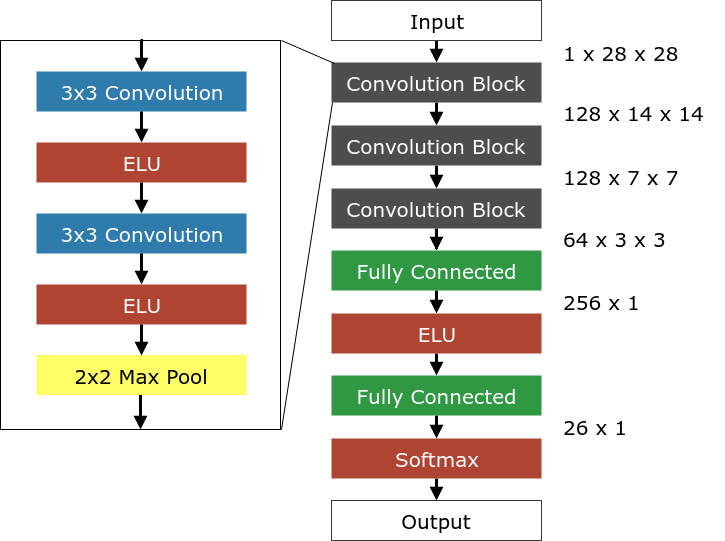
\includegraphics[height=0.25\paperwidth]{graphics/nets/CNN13}
        \caption{\textit{Model of DeepCNN}}
        \label{fig:deepCNN_model}
    \end{subfigure}
    \begin{subfigure}[b]{0.5\textwidth}
        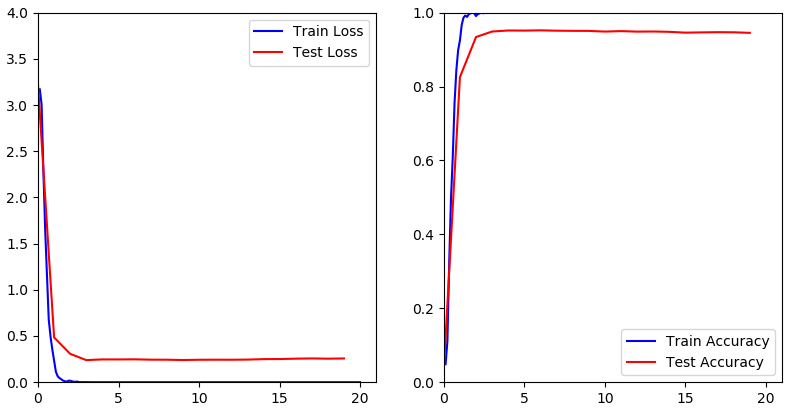
\includegraphics[height=0.25\paperwidth]{graphics/nets/CNN13_Results}
        \caption{\textit{Results on DeepCNN}}
        \label{fig:deepCNN_results}
    \end{subfigure}
    \caption{\textit{Subplot \ref{fig:deepCNN_model} visualizes all layers of the DeepCNN model. Subplot \ref{fig:deepCNN_results} displays the train and test losses (left plot), as well as the train and test accuracies (right plot) as a function of the trained epochs.}}\label{fig:deepCNN}
\end{figure*}

In order to improve our results, we designed the DeepCNN. This neural net has in comparison with the SimpleCNN more convolutional layers, more pooling layers and more neurons in the fully connected layers. The convolution part is structured in convolution blocks, each consisting of two 3x3 convolution layers, two ELU functions and one 2x2 max pool layer. The latter reduces the last two dimensions by the factor of two. The DeepCNN contains three cascaded convolution blocks with two fully connected layers subsequently. We experienced with many variations of the DeepCNN in order to find the best net layout. Surprisingly, the best net does reduce the number of kernels in deeper layers. For a schematic see figure \ref{fig:deepCNN_model}. 

The evaluation for this training can be found in figure \ref{fig:deepCNN_results}. We achieved 94.7 \% train accuracy after only 4 epochs. The following epochs did neither improve nor worsen the test accuracy. 

\subsection{DeepCNN with Data Augmentation}\label{sec:deepCNN_augmented}

\begin{figure*}
     \centering
     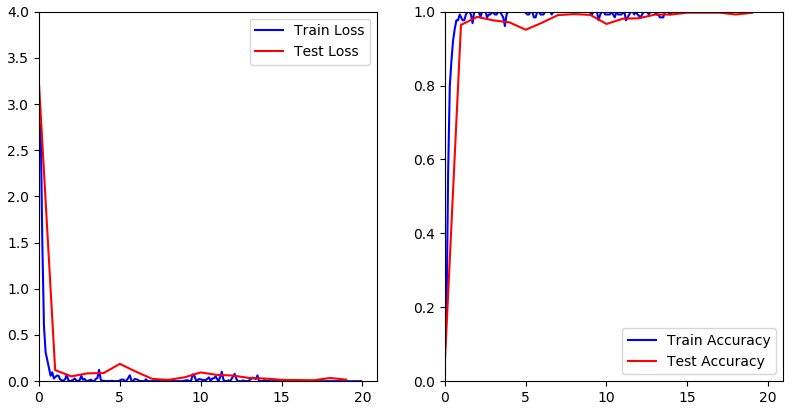
\includegraphics[height=0.25\paperwidth]{graphics/nets/CNN13_with_Augmentation_Results}
     \caption{\textit{Left plot displays the train and test losses for the DeepCNN with prior application of the random crop data augmentation as a function of the trained epochs. The right plot displays the train and test accuracies.}}
     \label{fig:deepCNN_augmented}
\end{figure*}

We applied a data augmentation technique to the train dataset in order to improve the generalization of the DeepCNN. We chose the random crop augmentation (see section [TODO]), which produces the results in figure \ref{fig:deepCNN_augmented}. After 20 epochs we reached 99.7 \% test accuracy. During the learning phase the test accuracy decreased multiple times for a short period before reaching the maximum. In the following section we apply regularization techniques such as batch normalization and dropout to reduce this effect and to learn faster. 

\subsection{DeepCNN with Batch Normalization and Dropout}\label{sec:deepCNN_regularized}
\begin{figure*}
    \centering
    \hspace{-1cm}
    \begin{subfigure}[b]{0.4\textwidth}
        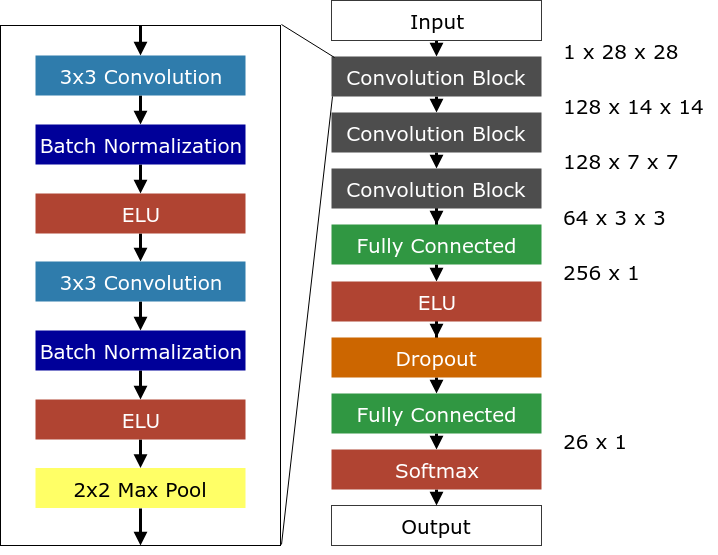
\includegraphics[height=0.25\paperwidth]{graphics/nets/CNN13_with_BN}
        \caption{\textit{Model of DeepCNN with batch normalization and dropout}}
        \label{fig:deepCNN_regularized_model}
    \end{subfigure}
    \begin{subfigure}[b]{0.5\textwidth}
        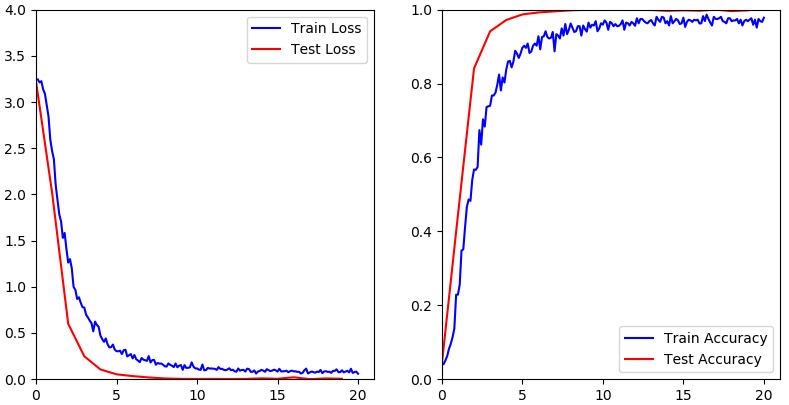
\includegraphics[height=0.25\paperwidth]{graphics/nets/CNN13_with_BN_Results}
        \caption{\textit{Results on DeepCNN with batch normalization and dropout}}
        \label{fig:deepCNN_regularized_results}
    \end{subfigure}
    \caption{\textit{Subplot \ref{fig:deepCNN_regularized_model} visualizes all layers of the DeepCNN model with batch normalization and dropout. Subplot \ref{fig:deepCNN_regularized_results} displays the train and test losses (left plot), as well as the train and test accuracies (right plot) as a function of the trained epochs.}}\label{fig:deepCNN_regularized}
\end{figure*}

We modified the convolution block by adding batch normalization \cite{ioffe2015batch} after each convolution layer. Batch normalization is applied to each mini batch in order to normalize the data distribution between layers. Thus, allowing larger learning rates, gives more robustness against parameter initialization and reduces saturation of layers. \cite{ioffe2015batch}. In order to increase the generalization of our fully connected layers we added dropout to the first one during the training phase. This technique randomly selects neurons and set their output to zero. 

In order to find the best hyperparameters we implemented a grid search, which trained and evaluated the whole network for all  combination of hyperparameters given our options. The varied hyperparameters are batch size, learning rate, weight decay, dropout probability and the usage of batch normalization.

Figure \ref{fig:deepCNN_regularized_results} shows the train/test losses and accuracies throughout the training. Due to the dropout in the training phase, the train loss (blue line) is now higher than the test loss (red line). After 9 epochs we reached a train accuracy of 100 \% using a dropout probability of 95 \%. This high dropout probability implies, that our first fully connected layer of our neural net is too big and might would work with less neurons as well. For comparison, we viewed the leaderboard of the similar task digit classification on the MNIST dataset. Our network achieved an error of 0 \%, while the seemingly easier task due to the number of classes has 0.21 \% as its best. This has two reasons. Firstly, the MNIST dataset contains digits, which are not clearly written and therefore cannot be identified uniquely even for humans, while the SignlanuageMNIST dataset only contains well-defined characters. Secondly, our dataset was created from 1794 original images from 7 different persons. This results in a great similarity between the train and test images and therefore yields in an easier classification task.

\section{Evaluation}
\subsection{Validation on custom dataset}
\begin{figure}[t]
     \centering
     \begin{tabular}{ccc}
          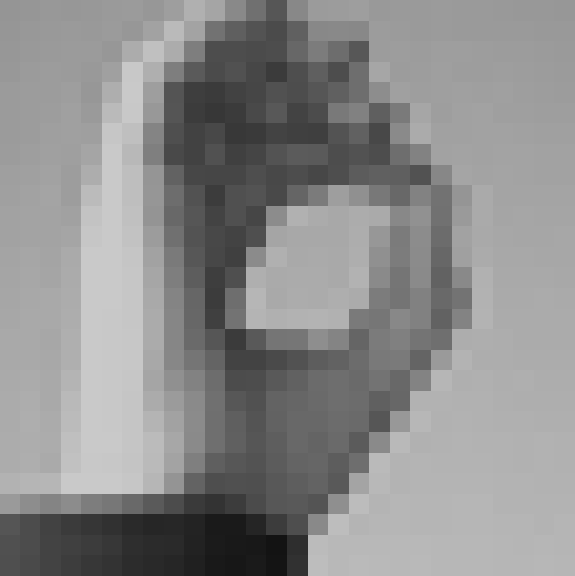
\includegraphics[width=.25\linewidth]{graphics/custom_dataset/orig0}&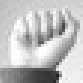
\includegraphics[width=.25\linewidth]{graphics/custom_dataset/orig1}&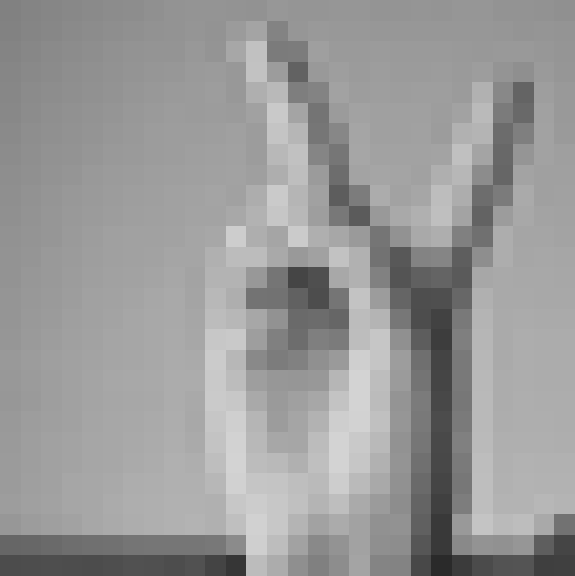
\includegraphics[width=.25\linewidth]{graphics/custom_dataset/orig2} \\
          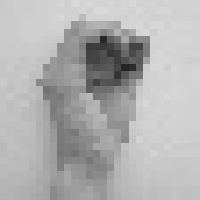
\includegraphics[width=.25\linewidth]{graphics/custom_dataset/custom0}&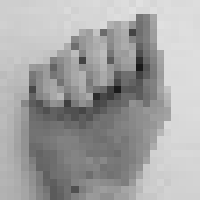
\includegraphics[width=.25\linewidth]{graphics/custom_dataset/custom1}&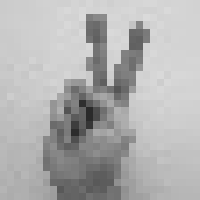
\includegraphics[width=.25\linewidth]{graphics/custom_dataset/custom2}
     \end{tabular}
     \caption{\textit{Exemplary images from original (top row) and custom (bottom row) datasets.}}
     \label{fig:custom_dataset} 
\end{figure}
To determine the trained model's capacity to generalize to real-world examples beyond those of the provided test set, we created a small custom dataset of 60 images of sign language gestures made by our own hands in front of a white background. To keep the scenario as realistic as possible, preprocessing of the images was constrained to grayscale conversion, cropping and rescaling to the expected size of 28x28 pixels. Three of the images in the custom dataset, together with corresponding images from the provided test set, are shown in figure \ref{fig:custom_dataset}. Despite its capability of correctly classifying every image in the provided test set, the model failed to correctly classify a single image from the custom dataset. The poor performance of the classifier on real-world data indicates that the model did not learn salient features for classifying ASL hand gestures in general, but instead learned features only relevant to these particular training and test sets. To test this hypothesis, we chose to generate human-interpretable visual representations of the learned features. In the literature, several approaches for visualizing the features learned by neural networks in general and convolutional neural networks in particular have been proposed \cite{Qin2018}. PyTorch implementations of multiple neural network visualization algorithms are provided in the repository \textit{pytorch-cnn-visualizations} \cite{Ozbulak2018}, from which we used and slightly adapted the visualization of convolutional filters described in section \ref{sec:filter_visualization} as well as the gradient class-activation mapping (GradCAM) shown in section \ref{sec:gradcam}.

\subsection{Visualization of filters}
\label{sec:filter_visualization}
\begin{figure}[t]
     \centering
     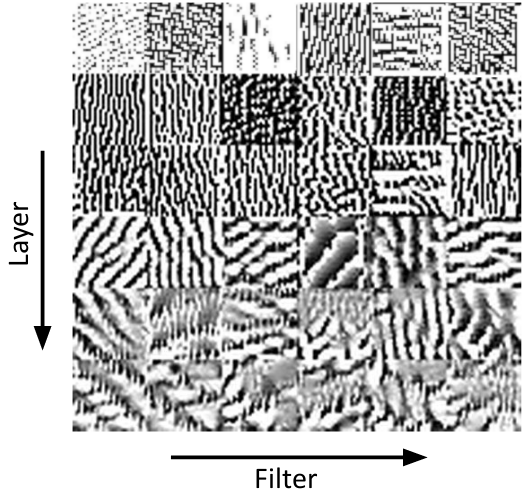
\includegraphics[width=.9\linewidth]{graphics/filters}
     \caption{\textit{Input images optimizing convolution outputs for the filters of the six convolutional layers of the final model. Only a subset of all layers of each filter is shown.}}
     \label{fig:filters}
\end{figure}
A common visualization technique for understanding the features learned by a convolutional neural network is to display the weights in the filters of the convolutional layers. Filters at the first layers tend to be easily interpretable, usually as pattern or edge detectors, while the filters of deeper layers become less interpretable. A different approach is to visualize the optimal input image with respect to a given convolution via gradient ascent in the input space \cite{Erhan2009}. This way, we do not visualize the weights, but rather the \enquote{archetypical feature} which maximizes the output of a given filter. Algorithm \ref{alg:filter_visualization} shows a PyTorch-based implementation of the optimization-based filter visualization.

\begin{algorithm}
     \caption{Convolution Input Optimization}\label{alg:filter_visualization}
     \begin{lstlisting}[language=Python]
hook_pytorch_layer(model)
x = random_tensor(shape=(224, 224, 3))
optimizer = torch.optim.Adam([x])
for i in range(30):
  optimizer.zero_grad()
  for j, layer in enumerate(model):
    x = layer(x) # forward pass
    if j == selected_layer:
      break # forward hook function has been triggered
    loss = -torch.mean(conv_output)
    loss.backward()
    optimizer.step()
     \end{lstlisting}
\end{algorithm}

A PyTorch layer hook function is registered to save the output (here: \texttt{conv\_output}) of the convolution with a specified filter at a specified layer (here: \texttt{selected\_layer}). An \texttt{Adam} optimizer \cite{Kingma2014} is initialized for a random image. In each of a total of 30 iterations, the optimizer's gradients are reset and the current version of the input image is forward-propagated through the network up to the specified layer, at which point the registered hook function stores the convolution output in \texttt{conv\_output}. The loss (the negative mean of \texttt{conv\_output}) is then backpropagated through the network and the image is updated by the optimizer.\\
A subset of the resulting images is shown in figure \ref{fig:filters}. In the first layers, the outputs of the convolutions are maximized for high-frequency inputs with different primary orientations. Filters in deeper layers respond more strongly to lower-frequency patterns. This indicates that filters in deeper layers respond more strongly to larger features of the image and suggests that the network has learned to extract features beyond the high-frequency noise characteristics of the training set.

\subsection{GradCAM visualization}
\label{sec:gradcam}
\begin{figure}[t]
     \centering
     \begin{tabular}{ccc}
          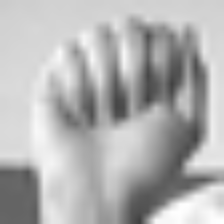
\includegraphics[width=.25\linewidth]{graphics/gradcam/layer1/0_original}&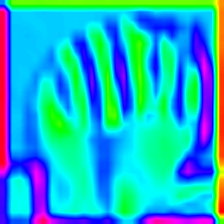
\includegraphics[width=.25\linewidth]{graphics/gradcam/layer1/0_map}&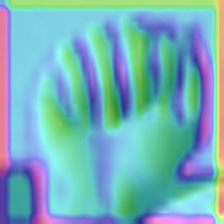
\includegraphics[width=.25\linewidth]{graphics/gradcam/layer1/0_overlaid} \\
          
\includegraphics[width=.25\linewidth]{graphics/gradcam/layer3/0_original}&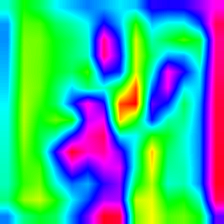
\includegraphics[width=.25\linewidth]{graphics/gradcam/layer3/0_map}&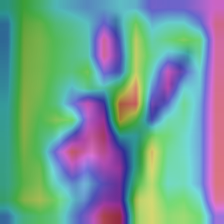
\includegraphics[width=.25\linewidth]{graphics/gradcam/layer3/0_overlaid} \\
          
\includegraphics[width=.25\linewidth]{graphics/gradcam/layer6/1_original}&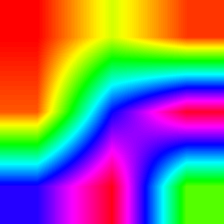
\includegraphics[width=.25\linewidth]{graphics/gradcam/layer6/1_map}&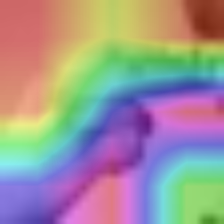
\includegraphics[width=.25\linewidth]{graphics/gradcam/layer6/1_overlaid} \\
          \textit{(a) Original} & \textit{(b) GradCAM} & \textit{(c) Overlaid}
     \end{tabular}
     \caption{\textit{GradCAM visualization of learned features for convolutional layers 1, 3 and 6 (1\ts{st}, 2\ts{nd} and 3\ts{rd} row respectively). The visualizations in column (c) are produced by overlaying the original image (a) with its GradCAM (b).}}
     \label{fig:gradcam}
\end{figure}
While the visualizations of optimal convolution inputs of section \ref{sec:filter_visualization} indicate that the network learned something other than noise, it does not give any indication whether the learned features are meaningful in the context of hand gesture recognition. To that end, we used the gradient class-activation mapping (GradCAM) algorithm \cite{Selvaraju2016} which generates a heat map indicating the importance of every pixel in the classification of an image. Unlike the generic visualization of optimal convolution inputs above, GradCAM is \textit{class-discriminative}: It visualizes how much each pixel contributed to the model's decision to classify an image into a particular class. Consequently, for an image of the gesture for the letter \enquote{A}, we expect the gradient class-activation map to highlight different regions of the hand than for an image of the gesture for the letter \enquote{V}, because different parts of the hand carry the salient information: The \enquote{A-ness} of an image of a hand is mainly captured by the four parallel fingers curled into a fist, while the \enquote{V-ness} of an image of a hand is mainly determined by the positions of the tips of the index and middle fingers.\\
\begin{algorithm}
     \caption{Gradient Class-Activation Mapping}
     \label{alg:gradcam}
     \begin{enumerate}
          \item Compute the gradient $\frac{\partial y^c}{\partial A^k}$ of the class score $y^c$ for class $c$ with respect to the feature maps $A^k$ of the given convolutional layer
          \item Compute the \textit{neuron importance weights}\\ $\alpha^c_k = \frac{1}{Z} \sum_i \sum_j \frac{\partial y^c}{\partial A^k_{ij}}$
          \item Compute the class-discriminative localization map\\
          $L^c_{GradCAM} = ReLU(\sum_k \alpha_k^c A^k)$
     \end{enumerate}
\end{algorithm}
Algorithm \ref{alg:gradcam} summarizes the GradCAM algorithm. Note that the neuron importance weights $\alpha_k^c$ are the result of global average pooling of the gradients and encode the importance of feature map $A^k$ for the decision for class $c$. $Z = i*j$ denotes the size of the feature map. The ReLU activation of the weighted sum in the third step is required to only keep pixels whose intensity should be \textit{increased} to increase $y^c$.\\
Exemplary results of computing the gradient class-activation maps for images from the test dataset are shown in figure \ref{fig:gradcam}. It is noteworthy that the size of the considered regions increases with the depth of the layers. In layers 3 and 6, the salient features (the fingertips for the \textit{V}, the orientation of the fingers for the \textit{H}) are captured. The first row of figure \ref{fig:gradcam} shows that in the first layer, edges are primarily considered, which is expected. However, only dark edges on the right side of the fingers are highlighted. This indicates that the network at least partially learned to consider the lighting characteristics of the image in the first layers, which is problematic because the hands in the images of the provided training and test sets are illuminated exclusively from the left. Real-world examples such as our custom dataset will not necessarily share these lighting characteristics. Figure \ref{fig:gradcam_custom} shows an exemplary GradCAM visualization of a misclassified instance from the custom dataset. Interestingly, the considered areas look similar to those of the test dataset, but the salient region for the last convolutional layer is much larger than in the corresponding image in figure \ref{fig:gradcam}, likely because the earlier layers of the feature extractor failed to find expected features (such as dark edges on the right side of the fingers). This supports our hypothesis that the uniformity of the training and test sets prevents the model from generalizing well to real-world examples from a different distribution: The learned features are salient for the training and test sets, but on the custom dataset, they are not present and the model lacks the basis for a correct classification.
\begin{figure}[t]
     \centering
     \begin{tabular}{cccc}
          
\includegraphics[width=.2\linewidth]{graphics/gradcam/custom_dataset/v_original}&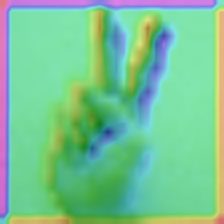
\includegraphics[width=.2\linewidth]{graphics/gradcam/custom_dataset/v_l1}&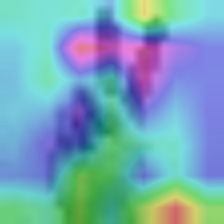
\includegraphics[width=.2\linewidth]{graphics/gradcam/custom_dataset/v_l3}&
          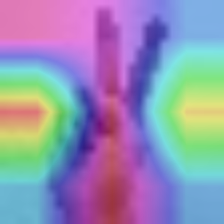
\includegraphics[width=.2\linewidth]{graphics/gradcam/custom_dataset/v_l5}\\
          \textit{Original} & \textit{Layer 1} & \textit{Layer 2} & \textit{Layer 3}
     \end{tabular}
     \caption{\textit{GradCAM visualization for a misclassified image from the custom dataset.}}
     \label{fig:gradcam_custom}
\end{figure}

\section{Conclusion and outlook}
Considering the implementation and evaluation of our model, several relevant conclusions can be drawn.\\
First, it is interesting to observe that for this particular problem, test accuracies exceeding [TODO]\% can be reached with a very simple neural network consisting of only one convolutional layer and two linear layers without regularization [TODO Note: L2 Regularization was used by default from the optimizer]. With a relatively simple deep model containing three convolutional and three fully connected layers, test accuracies exceeded [TODO]\% without any optimizations. This illustrates the particular suitability of convolutional neural networks for image classification in general as well as the suitability of the architecture combining convolutional feature extractors and fully connected classifiers for the particular task of hand gesture recognition.\\
Second, we observed that while a high-performing network architecture and parameterization could be found relatively quickly, a large amount of fine-tuning both of the architecture and the parameters was required to reach test accuracies exceeding 98\%. Somewhat surprisingly, grid search proved to be less effective in maximizing test accuracy than manual parameter tuning due to the high dimensionality of the parameter space. State-of-the-art approaches for automatic architecture and parameter search solve this problem by leveraging reinforcement learning \cite{Zoph2016}, dimensionality reduction \cite{Hinz2018} or massive parallelization \cite{Li2018}.\\
Lastly, and probably most significantly, we observed that the capacity of the trained model to generalize to test instances from different distributions at least partly depends on the variance of the training set. In our case, the fact that the training dataset featured only seven different hands and was generated by data augmentation from only 1704 original images, all of which share very similar backgrounds and lighting characteristics, caused the network to learn at least some characteristics of the dataset irrelevant for the actual classification of hand gestures, despite heavy regularization efforts and additional data augmentation during training. Along the same lines, we observed that a high classification accuracy on the test set is not a measure of true generalization capacity if the test set is drawn from the same or a very similar distribution as the training set.\\
\subsection{Future work}
Several approaches can be taken to improve the generalization capacity of our model. First, the neural network architecture can be modified to increase, instead of decrease, the filter size in deeper layers [TODO: Why would we want this exactly?] Second, the very high dropout probability of our network could likely be reduced, which would then permit a smaller network size and consequently, by the reduced number of parameters, would be less likely to overfit on the particularities of the training (and test) datasets. Third, the variance of the training data could be increased either by incorporating a larger custom dataset into the training data or by more aggressive data augmentation.

\bibliography{references}
\end{document}

